\documentclass[a4paper,12pt]{article}
\usepackage[backend=bibtex]{biblatex}
%\addbibresource{myBib.bib}
\usepackage{siunitx}
\usepackage{microtype}
\usepackage{float}
\usepackage{graphicx}
\usepackage{bm}
\usepackage{amsmath}
\usepackage{parskip}
\usepackage{longtable}
\usepackage{enumerate}
\graphicspath{}
\usepackage{geometry}  % for CUED specifications
\usepackage{tikz}
\usetikzlibrary{shapes,arrows,positioning,calc}
\usepackage{amssymb}
\usepackage{hyperref}
\usepackage{cleveref}
\usepackage{titlesec}
\newcommand{\sectionbreak}{\clearpage}
\title{Linear State Space Control Theory}
\date{June 4, 2015}
\author{Anas Syed}
\begin{document}
\maketitle
\tableofcontents
\newpage
\section{Introduction}
This document will introduce linear state space control theory for multiple input multiple output (MIMO) systems. The aim of this is to provide engineering students with an alternative set of notes which explains concepts with more details and less assumptions about their knowledge.
\subsection{Prerequisites}
\begin{enumerate}
  \item \textbf{Linear Algebra}
    \begin{itemize}
      \item Vector Spaces
      \item Matrix Algebra (inversion, determinant)
      \item Concept of rank
      \item Concept of row, column, null and left null space
      \item Eigendecomposition
    \end{itemize}
  \item \textbf{Linear dynamical systems}
  \item \textbf{Linear single input single output control theory}
    \begin{itemize}
      \item PID control
      \item Bode Plots
      \item Nyquist diagrams
      \item Nyquist stability criterion
      \item Pole-zero analysis of systems
    \end{itemize}
  \item \textbf{Integral Transforms}
    \begin{itemize}
      \item Fourier Transform
      \item Laplace Transform and its application to describing linear systems
    \end{itemize}
  \item \textbf{Ordinary differential equations}
  \item \textbf{Convolution}
\end{enumerate}
\section{State space description}
\subsection{Assumptions}
\begin{figure}[H]
  \centering
  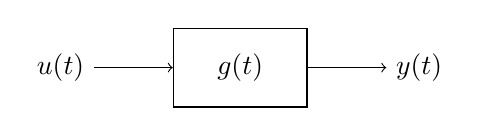
\begin{tikzpicture}
    \node (input) [] {$u(t)$};
    \node (process) [right =of input, rectangle, minimum width=0.14\textwidth, minimum height=1cm,text centered, draw=black] {$g(t)$};
    \node (output) [right =of process] {$y(t)$};
    \draw [->] (input) -- node[anchor=south] {} (process.west) ;
    \draw [->] (process.east) -- node[anchor=south] {} (output);
  \end{tikzpicture}
  \caption{A system in the time domain. $u(t) \in \mathbb{R}^m$, $y(t) \in \mathbb{R}^p$ and $g(t) \in \mathbb{R}^{p \times m}$.}
  \label{fig:simpleSystemTime}
\end{figure}

\begin{figure}[H]
  \centering
  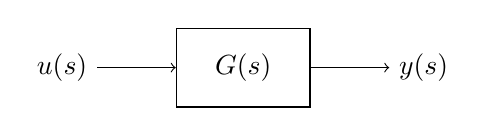
\begin{tikzpicture}
    \node (input) [] {$u(s)$};
    \node (process) [right =of input, rectangle, minimum width=0.14\textwidth, minimum height=1cm,text centered, draw=black] {$G(s)$};
    \node (output) [right =of process] {$y(s)$};
    \draw [->] (input) -- node[anchor=south] {} (process.west) ;
    \draw [->] (process.east) -- node[anchor=south] {} (output);
  \end{tikzpicture}
  \caption{A system in the Laplace domain. $u(s) \in \mathbb{R}^m$, $y(s) \in \mathbb{R}^p$ and $G(s) \in \mathbb{R}^{p \times m}$.}
  \label{fig:simpleSystemLaplace}
\end{figure}
\Cref{fig:simpleSystemTime} shows the block diagram of a system in the time domain. For all theory derived in this course, we make three key assumptions. Before you apply any of this theory to a real world system, you must make sure it satisfies the following three conditions (most systems do not):
\subsubsection{Linearity}
Consider the system $g(t)$ in \cref{fig:simpleSystemTime}. If an

fhwiehf
\subsubsection{Representable by ordinary differential equations}

\subsubsection{Time invariance}
\end{document}
